\documentclass{article}

\usepackage{graphicx}
\usepackage{tikz}
\usepackage{tikzsymbols}
\usetikzlibrary{calc,patterns,shapes.geometric}
\pagestyle{empty}
\usepackage[margin=0pt]{geometry}
\geometry{papersize={14in,12in}}

\def\centerarc[#1](#2)(#3:#4:#5){\draw[#1] ($(#2)+({#5*cos(#3)},{#5*sin(#3)})$) arc (#3:#4:#5);}

\begin{document}
	\begin{figure}
		\centering
		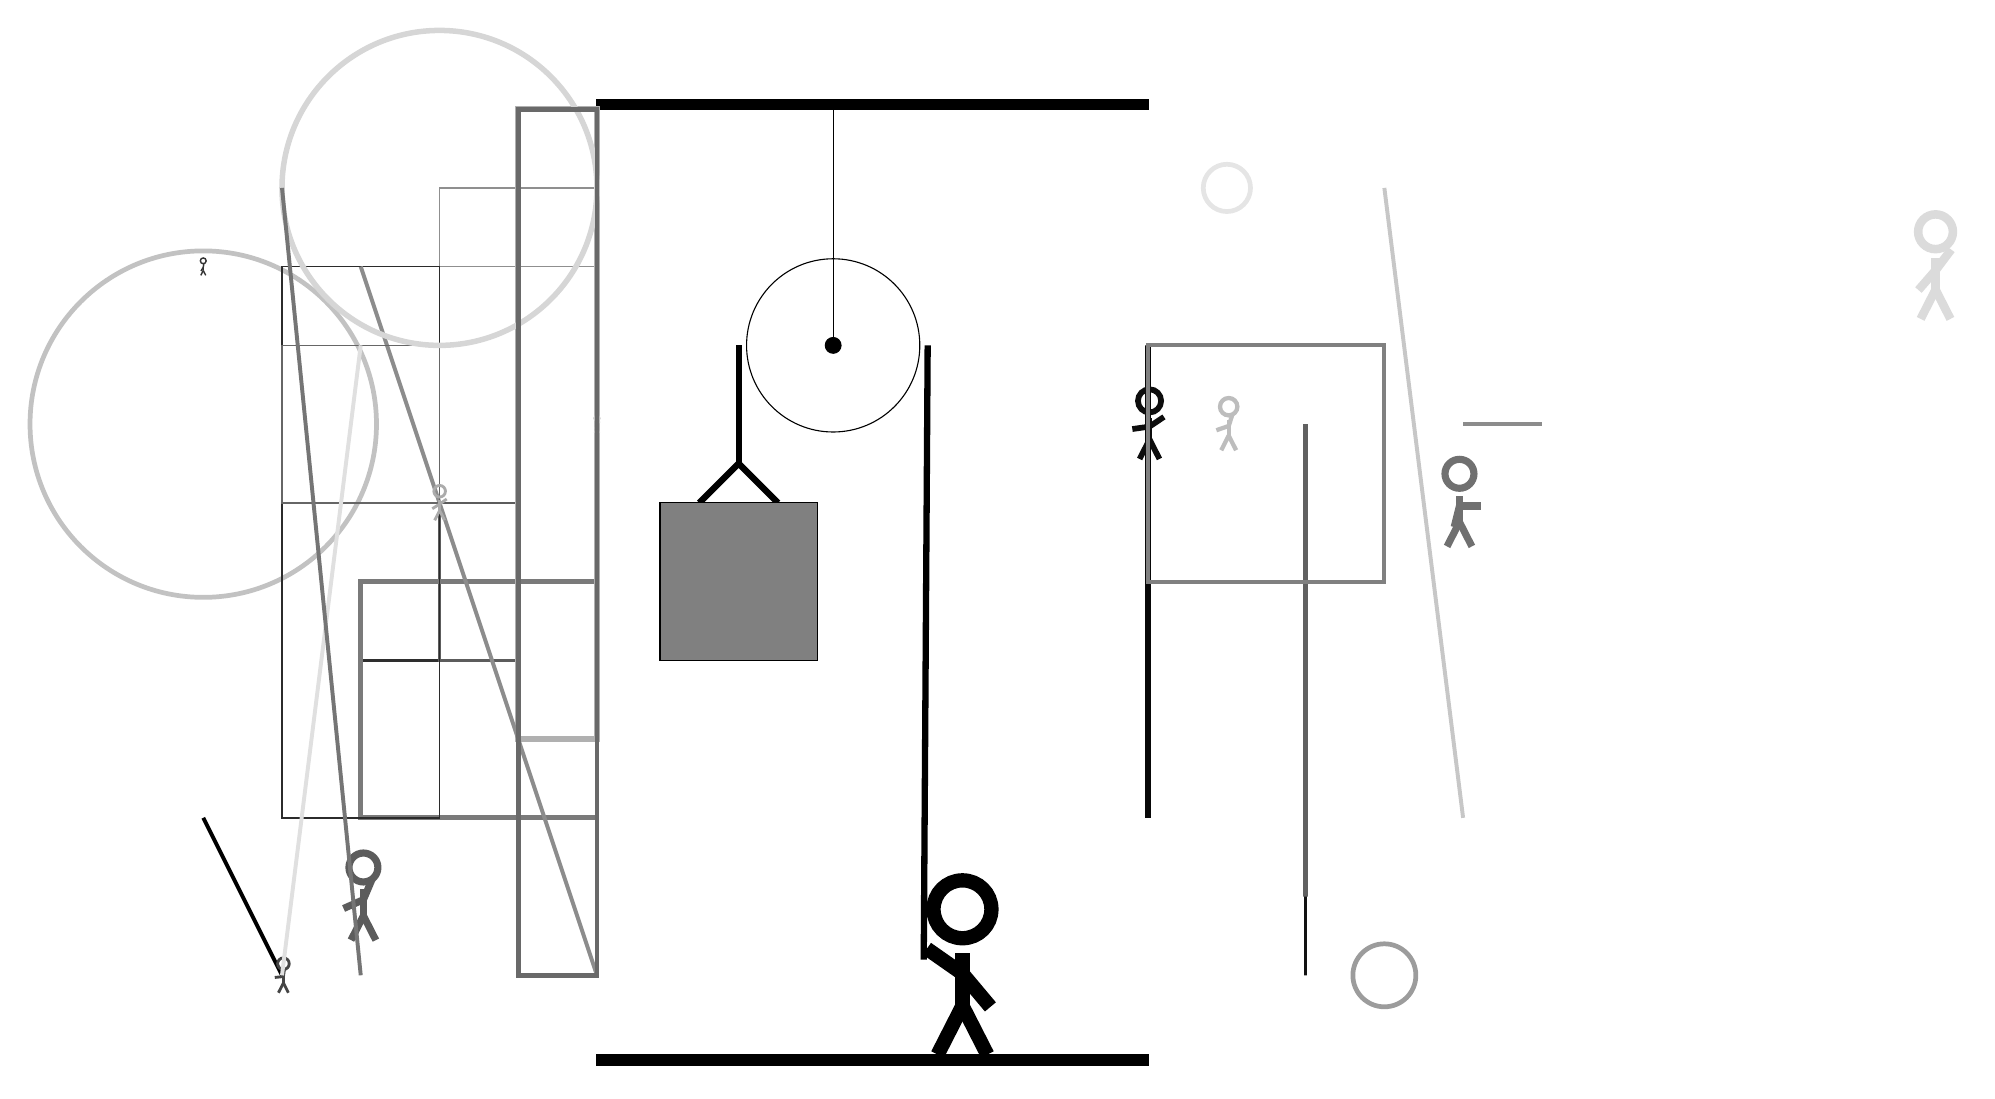
\begin{tikzpicture}
			%%%%% START %%%%%
			
			\draw[fill=black] (-2, 9) rectangle (5, 9.125);
			
			\draw (1, 6) circle (1.1);
			\draw[fill=black] (1, 6) circle (0.1);
			\draw (1, 9) -- (1, 6);
			
			\draw[line width=0.8mm] (-0.7, 4.0) -- (-0.2, 4.5) -- (0.3, 4.0);
			\draw[fill=black!50] (-1.2, 4.0) rectangle (0.8, 2.0);
			
			\draw[line width=0.5mm, color=black!100](-7, 0) -- (-6, -2);
			
			\draw [line width=0.6mm, color=black!10](6, 8) circle (0.3);
			\node[line width=0.2mm, color=black!56] at (9, 4) {\Strichmaxerl[5][76][0]};
			\draw[line width=0.2mm, color=black!44] (-4, 8) rectangle (-2, 7);
			\draw[line width=0.7mm, color=black!97] (5, 6) rectangle (5, 0);
			
			\draw[line width=0.4mm, color=black!82] (-3, 2) rectangle (-5, 3);
			
			\draw[line width=0.3mm, color=black!64] (-4, 2) rectangle (-3, 4);
			\draw [line width=0.6mm, color=black!24](-7, 5) circle (2.2);
			\node[line width=0.2mm, color=black!73] at (-6, -2) {\Strichmaxerl[2][6][82]};
			\draw[line width=0.6mm, color=black!52] (-2, 3) rectangle (-5, 0);
			\draw[line width=0.5mm, color=black!74](-3, 0) -- (-3, -1);
			
			\draw[line width=0.2mm, color=black!83] (-4, 0) rectangle (-6, 7);
			\node[line width=0.5mm, color=black!64] at (-5, -1) {\Strichmaxerl[5][24][67]};
			\draw[line width=0.7mm, color=black!31] (-2, 1) rectangle (-3, 9);
			\draw[line width=0.5mm, color=black!45](-5, 7) -- (-2, -2);
			\draw[line width=0.5mm, color=black!22](8, 8) -- (9, 0);
			\draw [line width=0.6mm, color=black!39](8, -2) circle (0.4);
			\node[line width=0.4mm, color=black!26] at (6, 5) {\Strichmaxerl[3][19][72]};
			\node[line width=0.4mm, color=black!95] at (5, 5) {\Strichmaxerl[4][8][34]};
			\node[line width=0.5mm, color=black!14] at (15, 7) {\Strichmaxerl[6][49][53]};
			\draw[line width=0.3mm, color=black!93] (7, 0) rectangle (7, -2);
			\draw[line width=0.2mm, color=black!60] (-4, 6) rectangle (-6, 4);
			\node[line width=0.4mm, color=black!80] at (-7, 7) {\Strichmaxerl[1][59][81]};
			\node[line width=0.6mm, color=black!33] at (-4, 4) {\Strichmaxerl[2][32][36]};
			\draw[line width=0.5mm, color=black!45](9, 5) -- (10, 5);
			\draw [line width=0.7mm, color=black!16](-4, 8) circle (2.0);
			
			\draw[line width=0.5mm, color=black!12](-6, -2) -- (-5, 6);
			\node[line width=0.5mm, color=black!25] at (-2, 5) {\Strichmaxerl[1][63][47]};
			
			\draw[line width=0.7mm, color=black!62] (7, -1) rectangle (7, 5);
			\draw[line width=0.5mm, color=black!54](-5, -2) -- (-6, 8);
			\draw[line width=0.5mm, color=black!50] (5, 6) rectangle (8, 3);
			
			\draw[line width=0.6mm, color=black!59] (-3, -2) rectangle (-2, 9);
			
			\draw[line width=0.8mm] (-0.2, 6) -- (-0.2, 4.5);
			\centerarc[line width=0.8mm](1, 6)(0:180:1.2000000000000002);
			\draw[line width=0.8mm](2.2, 6) -- (2.15, -1.8);
			
			\node at (2.6, -1.9) {\Strichmaxerl[10][-35][-50]};
			
			\draw[fill=black] (-2, -3) rectangle (5, -3.15);
			
			%%%%% END %%%%%
		\end{tikzpicture}
	\end{figure}	
\end{document}